
\newcommand{\printfigGraphTypes}{
    \begin{figure}
        \begin{subfigure}{.5\textwidth}
            \centering
            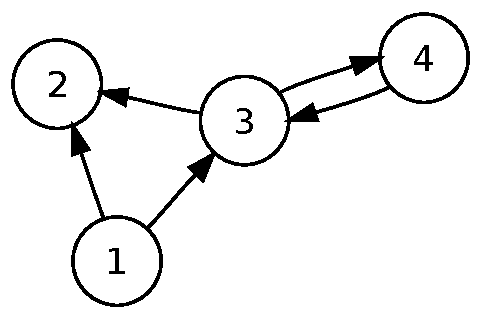
\includegraphics[width=.8\linewidth]{assets/images/Directed_graph_no_background.svg.pdf}
            \caption{Directed graph with cycle between nodes three and four.}
            \label{fig:directedgraph}
        \end{subfigure}
        \begin{subfigure}{.5\textwidth}
            \centering
            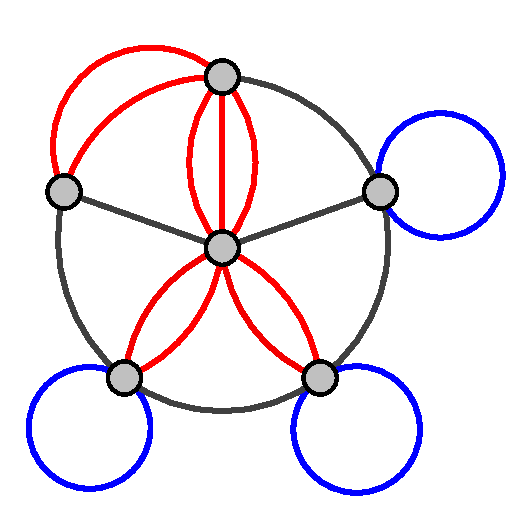
\includegraphics[width=.8\linewidth]{assets/images/Multi-pseudograph.svg.pdf}
            \caption{Multigraph with parallel edges and self-loops}
            \label{fig:multigraph}
        \end{subfigure}%
        \caption[]{Examples of first order graph symantics supported by Jaseci.\footnotemark}
        \label{fig:graph_examples}
    \end{figure}
    \footnotetext{Images credits to wiki contributers~\cite{wiki:Directed_graph_no_background.svg,wiki:Multi-pseudograph.svg}}
}


\newcommand{\printfigHelloWorldBaby}{
    \begin{figure}%{r}{0.5\textwidth}
        \centering
        
\includegraphics[width=.3\linewidth]{assets/images/hello_world_baby.jpg}
        \caption[]{World's youngest coder with valid HTML on shirt.\footnotemark}
        \label{fig:hello_baby}
    \end{figure}
    \footnotetext{Image credit to wiki contributer~\cite{wiki:hello_world_baby.jpg}}
}

\newcommand{\printtabPrecedence}{
    \begin{table}[t]
        \footnotesize
        \centering
        \begin{tabular}{l l l}
            \toprule
            \textbf{Rank} & \textbf{Symbol}                            & \textbf{Description}                           \\
            \midrule
            1             & \texttt{( ), [ ], ., ::, spawn}            & Parenthetical/grouping, node/edge manipulation \\
            2             & \texttt{\textasciicircum, []}              & Exponent,  Index                               \\
            3             & \texttt{*, /, \%  }                        & Multiplication, division, modulo               \\
            4             & \texttt{+, -}                              & Addition, subtraction                          \\
            5             & \texttt{==, !=, >=, <=, >, <, in, not in } & Comparison                                     \\
            6             & \texttt{\&\&, ||, and, or  }               & Logical                                        \\
            7             & \texttt{-->, <--, -[]->, <-[]-}            & Connect                                        \\
            8             & \texttt{=, +=, -=, *=, /=, := }            & Assignment                                     \\
            \bottomrule
        \end{tabular}
        \caption{Precedence of operations in Jac}
        \label{tab:jacprecedence} % Unique label used for referencing the table in-text
        %\addcontentsline{toc}{table}{Table \ref{tab:jacprecedence}} % Uncomment to add the table to the table of contents
    \end{table}
}

\newcommand{\printtabStrOps}{
    \begin{table}[t]
        \footnotesize
        \centering
        \rowcolors{1}{light-cyan}{light-gray}
        \begin{tabular}{l p{3cm} p{6cm}}
            \toprule
            \textbf{Op}                                           & \textbf{Args}                                                                                                                                                  & \textbf{Description} \\
            \midrule
            \lstinline{.str::upper}                               & none                                                                                                                                                           &                      \\
            \lstinline{.str::lower}                               & none                                                                                                                                                           &                      \\
            \lstinline{.str::title}                               & none                                                                                                                                                           &                      \\
            \lstinline{.str::capitalize}                          & none                                                                                                                                                           &                      \\
            \lstinline{.str::swap\_case}                          & none                                                                                                                                                           &                      \\
            \lstinline{.str::is\_alnum}                           & none                                                                                                                                                           &                      \\
            \lstinline{.str::is\_digit}                           & none                                                                                                                                                           &                      \\
            \lstinline{.str::is\_title}                           & none                                                                                                                                                           &                      \\
            \lstinline{.str::is\_upper}                           & none                                                                                                                                                           &                      \\
            \lstinline{.str::is\_lower}                           & none                                                                                                                                                           &                      \\
            \lstinline{.str::is\_space}                           & none                                                                                                                                                           &                      \\
            \lstinline{.str::load\_json}                          & none                                                                                                                                                           &                      \\
            \lstinline{.str::count}      & (\textbf{substr}, start, end)            & Returns the number of occurrences of a substring in the given string. Start and end specify range of indices to search                                                                \\
            \lstinline{.str::find}       &   (\textbf{substr}, start, end)            & Returns the index of first occurrence of the substring (if found). If not found, it returns -1. Start and end specify range of indices to search.                                     \\
            \lstinline{.str::split}      & \emph{optional} (separator, maxsplit) & Breaks up a string at the specified separator for maxsplit number of times and returns a list of strings. Default separators is ` ' and maxsplit is unlimited.                        \\
            \lstinline{.str::startswith}                          &                                                                                                                                                                &                      \\
            \lstinline{.str::endswith}                            &                                                                                                                                                                &                      \\
            \lstinline{.str::replace}                             &                                                                                                                                                                &                      \\
            \lstinline{.str::strip}                               & optional,                                                                                                                                                      &                      \\
            \lstinline{.str::lstrip}                              & optional,                                                                                                                                                      &                      \\
            \lstinline{.str::rstrip}                              & optional,                                                                                                                                                      &                      \\
            \bottomrule
        \end{tabular}
        \caption{String operations in Jac}
        \label{tab:strops} % Unique label used for referencing the table in-text
        %\addcontentsline{toc}{table}{Table \ref{tab:jacprecedence}} % Uncomment to add the table to the table of contents
    \end{table}
}

\newcommand{\printtabListOps}{
    \begin{table}[t]
        \footnotesize
        \centering
        \begin{tabular}{l l l}
            \toprule
            \textbf{Op}                     & \textbf{Args} & \textbf{Description}               \\
            \midrule
            \lstinline{.list::max}          & none          &                                    \\
            \lstinline{.list::min}          & none          &                                    \\
            \lstinline{.list::idx\_of\_max} & none          &                                    \\
            \lstinline{.list::idx\_of\_min} & none          &                                    \\
            \lstinline{.list::copy}         & none          & Returns a shallow copy of the list \\
            \lstinline{.list::deepcopy}     & none          & Returns a deep copy of the list    \\
            \lstinline{.list::sort}         & none          &                                    \\
            \lstinline{.list::reverse}      & none          &                                    \\
            \lstinline{.list::clear}        & none          &                                    \\
            \lstinline{.list::pop}          & optional,     &                                    \\
            \lstinline{.list::index}        &               &                                    \\
            \lstinline{.list::append}       &               &                                    \\
            \lstinline{.list::extend}       &               &                                    \\
            \lstinline{.list::insert}       &               &                                    \\
            \lstinline{.list::remove}       &               &                                    \\
            \lstinline{.list::count}        &               &                                    \\
            \bottomrule
        \end{tabular}
        \caption{List operations in Jac}
        \label{tab:listops} % Unique label used for referencing the table in-text
        %\addcontentsline{toc}{table}{Table \ref{tab:jacprecedence}} % Uncomment to add the table to the table of contents
    \end{table}
}

\newcommand{\printtabDictOps}{
    \begin{table}[t]
        \footnotesize
        \centering
        \begin{tabular}{l l l}
            \toprule
            \textbf{Op}                 & \textbf{Args} & \textbf{Description}                     \\
            \midrule
            \lstinline{.dict::items}    & none          &                                          \\
            \lstinline{.dict::copy}     & none          & Returns a shallow copy of the dictionary \\
            \lstinline{.dict::deepcopy} & none          & Returns a deep copy of the dictionary    \\
            \lstinline{.dict::keys}     & none          &                                          \\
            \lstinline{.dict::clear}    & none          &                                          \\
            \lstinline{.dict::popitem}  & none          &                                          \\
            \lstinline{.dict::values}   & none          &                                          \\
            \lstinline{.dict::pop}      &               &                                          \\
            \lstinline{.dict::update}   &               &                                          \\
            \bottomrule
        \end{tabular}
        \caption{Dictionary operations in Jac}
        \label{tab:dictops} % Unique label used for referencing the table in-text
        %\addcontentsline{toc}{table}{Table \ref{tab:jacprecedence}} % Uncomment to add the table to the table of contents
    \end{table}
}

\newcommand{\printtabJSAPI}{
    \rowcolors{1}{light-cyan}{light-gray}
    \begin{longtable}{l | p{10cm}}
        \toprule
        \rowcolor{white} \textbf{Interface} & \textbf{Parameters} \\
        \midrule
        \lstinline$walker callback$ & \lstinline$nd: node (*req), wlk: walker (*req), key: str (*req), ctx: dict (\{\}), _req_ctx: dict (\{\}), global_sync: bool (True)$ \\ \hline
\lstinline$walker summon$ & \lstinline$key: str (*req), wlk: walker (*req), nd: node (*req), ctx: dict (\{\}), _req_ctx: dict (\{\}), global_sync: bool (True)$ \\ \hline
\lstinline$walker register$ & \lstinline$snt: sentinel (None), code: str (), encoded: bool (False)$ \\ \hline
\lstinline$walker get$ & \lstinline$wlk: walker (*req), mode: str (default), detailed: bool (False)$ \\ \hline
\lstinline$walker set$ & \lstinline$wlk: walker (*req), code: str (*req), mode: str (default)$ \\ \hline
\lstinline$walker list$ & \lstinline$snt: sentinel (None), detailed: bool (False)$ \\ \hline
\lstinline$walker delete$ & \lstinline$wlk: walker (*req), snt: sentinel (None)$ \\ \hline
\lstinline$walker spawn create$ & \lstinline$name: str (*req), snt: sentinel (None)$ \\ \hline
\lstinline$walker spawn delete$ & \lstinline$name: str (*req)$ \\ \hline
\lstinline$walker spawn list$ & \lstinline$detailed: bool (False)$ \\ \hline
\lstinline$walker prime$ & \lstinline$wlk: walker (*req), nd: node (None), ctx: dict (\{\}), _req_ctx: dict (\{\})$ \\ \hline
\lstinline$walker execute$ & \lstinline$wlk: walker (*req), prime: node (None), ctx: dict (\{\}), _req_ctx: dict (\{\}), profiling: bool (False)$ \\ \hline
\lstinline$walker run$ & \lstinline$name: str (*req), nd: node (None), ctx: dict (\{\}), _req_ctx: dict (\{\}), snt: sentinel (None), profiling: bool (False)$ \\ \hline
\lstinline$user create$ & \lstinline$name: str (*req), global_init: str (), global_init_ctx: dict (\{\}), other_fields: dict (\{\})$ \\ \hline
\lstinline$alias register$ & \lstinline$name: str (*req), value: str (*req)$ \\ \hline
\lstinline$alias list$ & \lstinline$n/a$ \\ \hline
\lstinline$alias delete$ & \lstinline$name: str (*req)$ \\ \hline
\lstinline$alias clear$ & \lstinline$n/a$ \\ \hline
\lstinline$global get$ & \lstinline$name: str (*req)$ \\ \hline
\lstinline$global set$ & \lstinline$name: str (*req), value: str (*req)$ \\ \hline
\lstinline$global delete$ & \lstinline$name: str (*req)$ \\ \hline
\lstinline$global sentinel set$ & \lstinline$snt: sentinel (None)$ \\ \hline
\lstinline$global sentinel unset$ & \lstinline$n/a$ \\ \hline
\lstinline$object get$ & \lstinline$obj: element (*req), depth: int (0), detailed: bool (False)$ \\ \hline
\lstinline$object perms get$ & \lstinline$obj: element (*req)$ \\ \hline
\lstinline$object perms set$ & \lstinline$obj: element (*req), mode: str (*req)$ \\ \hline
\lstinline$object perms default$ & \lstinline$mode: str (*req)$ \\ \hline
\lstinline$object perms grant$ & \lstinline$obj: element (*req), mast: element (*req), read_only: bool (False)$ \\ \hline
\lstinline$object perms revoke$ & \lstinline$obj: element (*req), mast: element (*req)$ \\ \hline
\lstinline$graph create$ & \lstinline$set_active: bool (True)$ \\ \hline
\lstinline$graph get$ & \lstinline$gph: graph (None), mode: str (default), detailed: bool (False)$ \\ \hline
\lstinline$graph list$ & \lstinline$detailed: bool (False)$ \\ \hline
\lstinline$graph active set$ & \lstinline$gph: graph (*req)$ \\ \hline
\lstinline$graph active unset$ & \lstinline$n/a$ \\ \hline
\lstinline$graph active get$ & \lstinline$detailed: bool (False)$ \\ \hline
\lstinline$graph delete$ & \lstinline$gph: graph (*req)$ \\ \hline
\lstinline$graph node get$ & \lstinline$nd: node (*req), keys: list ([])$ \\ \hline
\lstinline$graph node set$ & \lstinline$nd: node (*req), ctx: dict (*req), snt: sentinel (None)$ \\ \hline
\lstinline$graph walk (cli only)$ & \lstinline$nd: node (None)$ \\ \hline
\lstinline$sentinel register$ & \lstinline$name: str (default), code: str (), code_dir: str (./), mode: str (default), encoded: bool (False), auto_run: str (init), auto_run_ctx: dict (\{\}), auto_create_graph: bool (True), set_active: bool (True)$ \\ \hline
\lstinline$sentinel pull$ & \lstinline$set_active: bool (True), on_demand: bool (True)$ \\ \hline
\lstinline$sentinel get$ & \lstinline$snt: sentinel (None), mode: str (default), detailed: bool (False)$ \\ \hline
\lstinline$sentinel set$ & \lstinline$code: str (*req), code_dir: str (./), encoded: bool (False), snt: sentinel (None), mode: str (default)$ \\ \hline
\lstinline$sentinel list$ & \lstinline$detailed: bool (False)$ \\ \hline
\lstinline$sentinel test$ & \lstinline$snt: sentinel (None), detailed: bool (False)$ \\ \hline
\lstinline$sentinel active set$ & \lstinline$snt: sentinel (*req)$ \\ \hline
\lstinline$sentinel active unset$ & \lstinline$n/a$ \\ \hline
\lstinline$sentinel active global$ & \lstinline$auto_run: str (), auto_run_ctx: dict (\{\}), auto_create_graph: bool (False), detailed: bool (False)$ \\ \hline
\lstinline$sentinel active get$ & \lstinline$detailed: bool (False)$ \\ \hline
\lstinline$sentinel delete$ & \lstinline$snt: sentinel (*req)$ \\ \hline
\lstinline$wapi$ & \lstinline$name: str (*req), nd: node (None), ctx: dict (\{\}), _req_ctx: dict (\{\}), snt: sentinel (None), profiling: bool (False)$ \\ \hline
\lstinline$architype register$ & \lstinline$code: str (*req), encoded: bool (False), snt: sentinel (None)$ \\ \hline
\lstinline$architype get$ & \lstinline$arch: architype (*req), mode: str (default), detailed: bool (False)$ \\ \hline
\lstinline$architype set$ & \lstinline$arch: architype (*req), code: str (*req), mode: str (default)$ \\ \hline
\lstinline$architype list$ & \lstinline$snt: sentinel (None), detailed: bool (False)$ \\ \hline
\lstinline$architype delete$ & \lstinline$arch: architype (*req), snt: sentinel (None)$ \\ \hline
\lstinline$master create$ & \lstinline$name: str (*req), global_init: str (), global_init_ctx: dict (\{\}), other_fields: dict (\{\})$ \\ \hline
\lstinline$master get$ & \lstinline$name: str (*req), mode: str (default), detailed: bool (False)$ \\ \hline
\lstinline$master list$ & \lstinline$detailed: bool (False)$ \\ \hline
\lstinline$master active set$ & \lstinline$name: str (*req)$ \\ \hline
\lstinline$master active unset$ & \lstinline$n/a$ \\ \hline
\lstinline$master active get$ & \lstinline$detailed: bool (False)$ \\ \hline
\lstinline$master self$ & \lstinline$detailed: bool (False)$ \\ \hline
\lstinline$master delete$ & \lstinline$name: str (*req)$ \\ \hline
\lstinline$master createsuper$ & \lstinline$name: str (*req), global_init: str (), global_init_ctx: dict (\{\}), other_fields: dict (\{\})$ \\ \hline
\lstinline$master allusers$ & \lstinline$num: int (0), start_idx: int (0)$ \\ \hline
\lstinline$master become$ & \lstinline$mast: master (*req)$ \\ \hline
\lstinline$master unbecome$ & \lstinline$n/a$ \\ \hline
\lstinline$config get$ & \lstinline$name: str (*req), do_check: bool (True)$ \\ \hline
\lstinline$config set$ & \lstinline$name: str (*req), value: str (*req), do_check: bool (True)$ \\ \hline
\lstinline$config list$ & \lstinline$n/a$ \\ \hline
\lstinline$config index$ & \lstinline$n/a$ \\ \hline
\lstinline$config exists$ & \lstinline$name: str (*req)$ \\ \hline
\lstinline$config delete$ & \lstinline$name: str (*req), do_check: bool (True)$ \\ \hline
\lstinline$logger http connect$ & \lstinline$host: str (*req), port: int (*req), url: str (*req), log: str (all)$ \\ \hline
\lstinline$logger http clear$ & \lstinline$log: str (all)$ \\ \hline
\lstinline$logger list$ & \lstinline$n/a$ \\ \hline
\lstinline$actions load local$ & \lstinline$file: str (*req)$ \\ \hline
\lstinline$actions load remote$ & \lstinline$url: str (*req)$ \\ \hline
\lstinline$actions load module$ & \lstinline$mod: str (*req)$ \\ \hline
\lstinline$actions list$ & \lstinline$name: str ()$ \\ \hline
\lstinline$jac build (cli only)$ & \lstinline$file: str (*req), out: str ()$ \\ \hline
\lstinline$jac test (cli only)$ & \lstinline$file: str (*req), detailed: bool (False)$ \\ \hline
\lstinline$jac run (cli only)$ & \lstinline$file: str (*req), walk: str (init), ctx: dict (\{\}), profiling: bool (False)$ \\ \hline
\lstinline$jac dot (cli only)$ & \lstinline$file: str (*req), walk: str (init), ctx: dict (\{\}), detailed: bool (False)$ \\ \hline

        \bottomrule
        \hiderowcolors
        \caption{Full set of core Jaseci APIs}
        \label{tab:jsAPI}
    \end{longtable}
}